\newcommand{\Mem}{\textit{Mem} }
\newcommand{\Equ}{\textit{Equ} }
\newcommand{\safe}{S}
\newcommand{\unsafe}{U}
\newcommand{\unknown}{?}
\newcommand{\exception}{E}
\newcommand{\timeout}{T.O.}
\newcommand{\unknownmark}{\ensuremath{^?}}
\newcommand{\wrongmark}{\ensuremath{^!}}

\chapter{Experiments}\label{ch:experiments}

This chapter presents our experimental results to justify the claims made in this paper. We evaluated the performance of our prototype in synthesize-and-verify mode using the recursive category from SV-COMP 2015 \cite{svcomp15} \cite{svcomp-benchmarks}. The recursive category consists of 24 non-trivial examples such as Ackermann, McCarthy 91, and Euclidean algorithms. Among the 24 examples, 8 of them contain an error. Moreover, we compared the performance of both modes using the recursive and array-examples categories from SV-COMP 2016 \cite{svcomp16} benchmarks. In this set of benchmarks, the array-examples category consists of 88 non-trivial examples demonstrating various operations on arrays of various sizes, whereas the recursive category in SV-comp 2016 has one file modified from buggy to bug-free. For the synthesize-and-verify mode, we ran the experiments with $\epsilon = 0.1, \delta = 0.9$ and size of a batched sample $k = 10$. We ran our prototype on each example three times in all experiments. The provided statistical data were calculated based on the average of the three runs unless explicitly stated otherwise. We set the timeout to 900 seconds to match the rules of SV-COMP.  

We submitted our prototype in direct mode to participate in the recursive and array-reach categories in SV-COMP 2016. Considering our straightforward approach and implementation, our score was surprisingly good. It is also possible to incorporate sophisticated heuristics and optimization techniques into our prototype in order to enhance its performance.

\section{Comparison of Learning Algorithms}\label{sec:compare_learning_algorithms}

We evaluated our approach with different automata learning algorithms implemented within the \textsc{libALF} library. There are five active online automata learning algorithms implemented in \textsc{libALF}: Angluin's $L^\ast$ \cite{Angluin87}, $L^\ast-columns$, Kearns/Vazirani (KV) \cite{KearnsV94}, Rivest/Schapire (RS) \cite{RivestS93}, and $NL^\ast$ \cite{BolligHKL09}. Among the search strategies provided by \textsc{Crest}, we chose the \emph{random branch} strategy. The experimental results are shown in Table \ref{table:compare_learning_algorithms}.

\begin{table}[h]
	\caption{Comparison of the learning algorithms}
	\label{table:compare_learning_algorithms}
	\centering
	\begin{tabular}{|l|l|l|l|l|l|}
		\cline{2-6}
		\multicolumn{1}{c|}{} & \multicolumn{5}{c|}{Algorithms} \\
		\cline{2-6}
		\multicolumn{1}{c|}{} & KV & $L^\ast$	& $L^\ast$-col & RS & $NL^\ast$ \\
		\hline
		Verified		&  15  & 9.67 &  10  & 11.33& 8.33 \\
		Bug found		&   6  & 6.33 &   6  & 6.33 &    6 \\
		\ \ by Bad  	&   4  & 4.67 &   4  &   3  & 4.33 \\
		\ \ by \CREST	&   2  & 1.67 &   2  & 3.33 & 1.67 \\
		\hline
		False positives	&   0  &   0  &   1  & 0.33 &    1 \\
		False negatives	&   2  & 1.67 & 1.33 & 1.67 &    1 \\
		Timeouts 		&   1  & 6.33 & 5.67 & 4.33 & 7.67 \\
		\hline
		\# of \Mem queries & 2896 & 8898 & 10071 & 15377 & 14463 \\
		\# of \Equ queries & 548 & 78 & 77 & 367 & 67 \\
		\hline
		Total time (s) & 2406 & 6668 & 6565 & 5786 & 7972 \\
		\Mem queries time & 30\% & 59\% & 58\% & 63\% & 70\% \\ 
		\hline
	\end{tabular}
\end{table}

The results show that KV is the algorithm with the best performance -- it solved 21 out of 24 examples. If the synthesize-and-verify mode of \PACMAN, equipped with KV learning algorithm, participated in the SV-COMP 2015, it would have won the \nth{2} place in the recursive category. The main reason for the difference in performance is that KV uses a tree-based data structure to store query results. Compared to other learning algorithms that use table-based data structures, KV requires much less number of membership queries to maintain the consistency of the tree-based data structure. For all learning algorithms except RS, the number of the error paths found by the emptiness test of the intersection of the conjecture and the bad automaton is more than that found by \CREST. In our experiments, the time spent on membership queries is often the performance bottleneck. Table \ref{table:compare_learning_algorithms} shows that membership queries took 30\% of the total execution time for KV, and at leat 58\% for the other learning algorithms. 

\section{Comparison of Search Strategies}\label{sec:compare_crest_strategies}

We also evaluated the performance of our algorithm against different \CREST search strategies. According to \cite{BurnimS08}, the most efficient search strategies are \emph{random branch} strategy (RBS for short) and \emph{control-flow directed} strategy (CDS for short). Therefore, we tested the performance of our prototype using these two strategies. We selected KV as the learning algorithm in this experiment. The results are shown in Table \ref{table:compare_crest_strategies}. 

\begin{table}[h]
	\caption{Comparison of search strategies of \CREST}
	\label{table:compare_crest_strategies}
	\centering
	\begin{tabular}{|l|l|l|}
		\cline{2-3}
		\multicolumn{1}{c|}{} & \multicolumn{2}{c|}{Search Strategy} \\
		\cline{2-3}
		\multicolumn{1}{c|}{} & \emph{RBS} & \emph{CDS} \\
		\hline
		Verified & 15 & 15 \\
		Bug found & 6 & 6 \\
		\hline
		False positives & 0 & 0 \\
		False negatives & 2 & 2 \\
		Timeouts & 1 & 1 \\
		\hline
		\# of \Mem queries & 2896 & 2362 \\
		\# of \Equ queries & 548 & 463 \\
		\hline
		Total time (s) & 2406 & 2013 \\ 
		Avg. time for one sample (s) & 0.75 & 0.82 \\
		\hline
	\end{tabular}
\end{table}

The table shows that although the average time for taking one sample with CDS is longer than with RBS, the total time is actually less. The main reason is that CDS explores untouched branching points more aggressively than RBS, yet requiring more overhead. Our experiments conform the results in \cite{BurnimS08}.

\section{Evaluation of \CREST with Restarts}\label{sec:eval_crest_restarts}

To justify our modification to the $\PAC$ness guarantee given in Section \ref{sec:stochastic_eq}, we show in the experiment below that running \CREST in batches does not decrease its bug-hunting capabilities. We compared the performance of \CREST with two different scenarios: 
\begin{enumerate}
	\item Restart \CREST after each $k$ decision vectors (note that in our experiment settings, $k = 10$).
	\item Never restart \CREST.
\end{enumerate}
We performed the experiment on the 8 programs that contain errors in the recursive category from SV-COMP 2015 benchmark suite, and calculated how many programs \CREST found a bug for within the timeout period. 

\begin{table}[h]
	\centering
	\caption{Evaluation of \CREST with and without restart}
	\label{table:eval_crest_restarts}
	\begin{tabular}{|l|l|l|}
		\cline{2-3}
		\multicolumn{1}{c|}{} & \multicolumn{2}{c|}{Settings} \\
		\hline
		Examples & \multicolumn{1}{c|}{\textit{Batch Size 10}} & \multicolumn{1}{c|}{\textit{Never Restart}} \\
		\hline
		Ackermann02 & batch 3 & iteration 14 \\
		Addition02 & batch 1  & iteration 2 \\
		Addition03 & Timeout & Timeout \\
		BallRajamani-SPIN2000 & batch 1 & iteration 1 \\
		EvenOdd03 & batch 1 & iteration 2 \\
		Fibonacci04 & batch 4 & iteration 2 \\
		Fibonacci05 & Timeout & Timeout \\
		McCarthy91 & batch 1 & iteration 2 \\
		\hline
		\multicolumn{3}{l}{
			\begin{tabular}[x]{@{}l@{}}
				$^\ast$The number of batches and the number of iterations used to find \\ 
				bugs are obtained respectively from the worst run in scenario 1 and \\
				from the best run in scenario 2.
			\end{tabular}
		}
	\end{tabular}
\end{table}

In Table \ref{table:eval_crest_restarts}, we chose RBS as the search strategy. We also used CDS to run the experiments and got very similar results. We list the worst result for scenario 1, and the best result for scenario 2 that we received in the three runs. With the experiment, we can confirm that the worst case in scenario 1 can still find, with a little overhead, all bugs found by the best case in scenario 2.  

\section{Evaluting Quality of Learned Automata}\label{sec:eval_learned_automata}

Besides the performance in terms of the running time, we also compared the quality of the learned automata produced by our prototype using the two strategies for the 15 successfully verified bug-free examples. To evaluate the quality of the learned automata, we ran \CREST with the given strategy to retrieve 1500 batched samples, then test how many of them are all accepted by the learned automaton. The average values of the runs are shown in Table \ref{table:eval_learned_automata}, where evaluation strategies are the strategies used to generate the batched samples under test. The table shows that the quality of the learned automata with the two strategies is almost identical. Also, observe that the guarantee of our procedure is that the sample coverage is higher than 90\%. Our experimental results show that the quality of the automata produced by our prototype under synthesize-and-verify mode matches the theoretical expectations. 

\begin{table}
	\centering
	\caption{Comparison of \CREST search strategies in terms of the quality of the learned automata}
	\label{table:eval_learned_automata}
	\begin{tabular}{|l|l|l|l|}
		\cline{3-4}
		\multicolumn{2}{c|}{} & \multicolumn{2}{c|}{\Equ query strategy} \\
		\cline{3-4}
		\multicolumn{2}{c|}{} & $RBS$ & $CDS$ \\
		\hline
		Evaluation & Accepted & 1487 & 1473 \\
		\cline{2-4}
		(RBS) & Ratio & 99.13\% & 98.2\% \\
		\hline
		\hline
		Evaluation & Accepted & 1489 & 1500 \\
		\cline{2-4}
		(CDS) & Ratio & 99.27\% & 100\% \\
		\hline
		\multicolumn{4}{l}{
			\begin{tabular}[x]{@{}l@{}}
				$^\ast$The total number of tested batches is 1500.
			\end{tabular}
		}
	\end{tabular}
\end{table}

Finally, we tested how many words generated by \CREST are not covered in the automata learned with KV algorithm and RBS. Again, we ran \CREST with RBS in two scenarios: 
\begin{enumerate}
	\item Restart \CREST after each $k$ decision vectors (note that in our experiment settings, $k = 10$).
	\item Never restart \CREST.
\end{enumerate}
For each of the 15 learned automata and each scenario, we generated 15000 decision vectors and checked how many of them are accepted by the automaton. In total, for scenario 1, we observed 1487 accepted batches of size 10 (for the total of 15000 tested vectors), yielding the correctness 99.13\%. For scenario 2, we observed 14977 accepted vectors, for the correctness 99.86\%. It is straightforward to observe that no matter what strategy we use, the learned automaton accepts over 99\% of the decision vectors produced by \CREST. 

\section{Comparing the Two Modes of \PACMAN}\label{sec:compare_learning_sampling}

In this section, we compare the two modes of \PACMAN, the \emph{synthesize-and-verify} and \emph{direct} mode. Moreover, we ran the direct mode of \PACMAN with two configurations: (1) use only the CDS in \CREST, and (2) use the CDS, RBS, and another search strategy named DFS in \CREST. We chose to use CDS instead of RBS because in the previous experiments CDS seemed to be the better performing search strategy. Also, in order to be fair, we splited the time limit of 900 seconds to three in configuration (2) of the direct mode, so that each strategy gets 300 seconds to run. We deemed a program to be proved correctly by configuration (2) of the direct mode only when the three strategies all report the program as bug-free. 

We executed this experiment on the recursive and array-examples benchmark sets in SV-COMP 2016. As stated before, the recursive benchmarks is generally identical to the 2015 version, except for one file changed from buggy to bug-free. The array-examples benchmarks is about the operations on large-sized arrays (up to 100000), such as examining the difference of two arrays, copying an array to another, and etc. The reason to run this experiment on SV-COMP 2016 benchmark suite instead of the 2015 version is because the $direct$ mode of \PACMAN is implemented after the 2016 benchmark suite's release. Since one of the aims of our implementation is to participate in SV-COMP 2016, it is only natural to use its announced benchmark suite. As for the previous experiments, their purpose were to justify the claims we made in the paper and to determine the algorithm/search strategy that performs the best, and therefore it is not a necessity to run these experiments on the latest, harder-to-solve benchmarks. 


\begin{table}[h]
	\centering
	\caption{Comparison different parameters in both modes with recursive category}
	\label{table:compare_param_recursive}
	\begin{tabular}{|l|l|l|l|}
		\hline
		$\epsilon = 0.1, \delta = 0.9$, & \multirow{2}{*}{Learning} & \multicolumn{2}{c|}{Sampling} \\
		\cline{3-4}
		batch size = 10 & & Single & Combined \\
		\hline
		Verified & 15 & 17 & 17 \\
		Bug found & 7 & 6 & 7 \\
		\hline
		False positives & 0 & 0 & 0 \\
		False negatives & 0 & 1 & 0 \\
		Timeouts & 2 & 0 & 0 \\
		\hline
		Total time (s) & 2579 & 514 & 1577 \\
		\hline
	\end{tabular}
	
	\bigskip
	
	\begin{tabular}{|l|l|l|l|}
		\hline
		$\epsilon = 0.004, \delta = 0.985$, & \multirow{2}{*}{Learning} & \multicolumn{2}{c|}{Sampling} \\
		\cline{3-4}
		batch size = 10 & & Single & Combined \\
		\hline
		Verified & 10 & 14 & 10 \\
		Bug found & 6 & 6 & 7 \\
		\hline
		False positives & 0 & 0 & 0 \\
		False negatives & 0 & 0 & 0 \\
		Timeouts & 8 & 4 & 7 \\
		\hline
		Total time (s) & 9064 & 7895 & 8644 \\
		\hline
	\end{tabular}
\end{table}

\clearpage
Table \ref{table:compare_param_recursive} is the results we obtained from running the experiment on the recursive category, with two different set of parameters: $\epsilon = 0.1, \delta = 0.9,$ with batch size of 10, and $\epsilon = 0.004, \delta = 0.985$ with batch size of 10. While the sampling-based approach have less overhead in terms of time usage, it can happen when they fail to reach bugs in the designated time and declare a buggy program as bug-free. However, with a set of parameters that is more extreme and gives better guarantees, sampling-based mechanisms can evade the false negatives by acquiring more samples. If the numbers of batched samples do not meet the requirements of the given parameters, then the sampling-based mechanisms report Unknown. Also note that with a more extreme setting, the configuration (2) of the sampling-based procedure degrades more drastice than configure (1). This is due to the fact that in configuration (2), all three strategies need to report a program as bug-free within 300 seconds in order to prove a program correct, whereas in configuration (1) only one search strategy is utilized, and the time limit is 900 seconds. 

\begin{table}[h]
	\centering
	\caption{Comparison different parameters in both modes with array-reach category}
	\label{table:compare_param_array}
	\begin{tabular}{|l|l|l|l|}
		\hline
		$\epsilon = 0.1, \delta = 0.9$, & \multirow{2}{*}{Learning} & \multicolumn{2}{c|}{Sampling} \\
		\cline{3-4}
		batch size = 10 & & Single & Combined \\
		\hline
		Verified & 5 & 57 & 57 \\
		Bug found & 17 & 16 & 16 \\
		\hline
		False positives & 0 & 0 & 0 \\
		False negatives & 0 & 9 & 9 \\
		Timeouts & 67 & 6 & 6 \\
		\hline
		Total time (s) & 60658 & 7657 & 7872 \\
		\hline
	\end{tabular}
	
	\bigskip
	
	\begin{tabular}{|l|l|l|l|}
		\hline
		$\epsilon = 0.004, \delta = 0.985$, & \multirow{2}{*}{Learning} & \multicolumn{2}{c|}{Sampling} \\
		\cline{3-4}
		batch size = 10 & & Single & Combined \\
		\hline
		Verified & 4 & 43 & 17 \\
		Bug found & 16 & 16 & 16 \\
		\hline
		False positives & 0 & 0 & 0 \\
		False negatives & 0 & 4 & 0 \\
		Timeouts & 68 & 25 & 55 \\
		\hline
		Total time (s) & 61674 & 44499 & 44584 \\
		\hline
	\end{tabular}
\end{table}

Table \ref{table:compare_param_array}, on the other hand, is the results we obtained from running the experiment on the array-reach category, also with the two sets of parameters. This category is in general more difficult to handle because of the decision vectors being very long due to the oftenly very large array sizes. For the learning-based proceudre, such behavior is more difficult to learn. Consequently, the performance of the learning-based procedure on this category is inferior to that on the recursive category. Sampling-based techniques do not rely on learning algorithms to give correctness guarantees, however they still suffer from the problem of identifying buggy program of bug-free. Observe that with the more extreme set of parameters, the number of false negatives (buggy programs identified as bug-free) decreased, but at the expense of more Unknowns (the Timeouts). 

After examining the results we obtained from the above experiments, we submitted \PACMAN in $direct$ mode to participate in the recursive and array-reach subcategories. Considering the straightforward approach and simplistic implementation, the score was beyond our expectation: we got \nth{5} place in the recursive subcategory, and \nth{4} in the array-reach. It is possible to add heuristics and mechanisms to detect the program's structures, so that the parameters can change on the fly depending on how complex the program-under-test really is. Also, it is also possible to utilize other samplers.

\begin{comment}

\section{Implementation}

\begin{figure}[t]
\begin{center}
\begin{tikzpicture}[
  node distance=1cm and 1.2cm, auto,>=latex', thick,
  decision/.style = {diamond, aspect=2, draw, align=center},
      data/.style = {draw,trapezium,trapezium left angle=70,
                     trapezium right angle=-70,minimum height=0.6cm},
     input/.style = {data, text width=18mm},
    output/.style = {rounded corners, draw, text width=1.5cm, align=center,
                     minimum height=0.7cm},
]
  % Nodes
  \node[decision] (analyzer) {Analyzer};
  \node[input, left=of analyzer] (rf_prog) {Intra-proc. Program};

  \node[data, above=.5cm of analyzer,text width=20mm] (proof) {Summary Candidates};

  \node[decision,above=.5cm of proof] (check) {Check};

  \node[input] (rc_prog) at (rf_prog |- check) {Recursive Program};
  \node[output, right=of analyzer] (unsafe) {FALSE};
  \node[output] (safe) at (check -| unsafe) {TRUE};

  % Edges
  \path[->]
    (rf_prog) edge (analyzer)
    (analyzer) edge node[anchor=north,sloped]{Error} (unsafe);

  \path[->]
    (rc_prog) edge 
      node[anchor=east]{Under-approx.}
    (rf_prog);

  \path[->]
    (analyzer) edge node[anchor=west]{Pass, Compute Summaries} (proof);
  \path[->]
    (proof) edge (check)
    (check) edge node[anchor=south,sloped]{Error, Refine} (rf_prog)
    (check) edge node[anchor=south,sloped]{Pass} (safe);

\end{tikzpicture}
\end{center}
\caption{The Execution Flow of \textsc{CPArec}}
\label{fig:flow}
\end{figure}

A prototype of our approach, \textsc{CPArec}, is implemented with
\textsc{CPAchecker} 1.2.11-svcomp14b as the underlying \method{BasicAnalyzer}.
The overall software architecture and execution flow is illustrated in
Figure~\ref{fig:flow}.
For all program transformations mentioned in
Chapter~\ref{ch:proving-via-transformation},
we benefit from the well-known front-end,
C Intermediate Language~(\textsc{CIL})~\cite{NeculaMRW02,cil}, to apply all required
transformations on C programs.
In addition, because \textsc{CPAchecker} does not support universal quantifiers
in the expression of an $\mathtt{assume}$ command,
we used \textsc{Redlog}~\cite{Dolzmann97,redlog} for quantifier elimination.

\textsc{CPArec} is available at~\url{https://github.com/fmlab-iis/cparec}.
The experiments in this paper is based on version v0.1-alpha.
The simplest way to execute \textsc{CPArec} is to first download the binary from
the web-site.
To setup the environment in Ubuntu 12.04 64-bit, JAVA Runtime, Python 2.7,
the Python Networkx package, and the Python PyGraphviz package are required.
Run following commands to install above packages in Ubuntu 12.04 64-bit:
\begin{lstlisting}[language=bash]
  sudo apt-get install openjdk-7-jre
  sudo apt-get install python python-networkx python-pygraphviz
\end{lstlisting}
To process a benchmark example \verb|program.c|, one should use the following script:
\begin{lstlisting}[language=bash]
  python <path_to_cparec>/cparec/main.py program.c
\end{lstlisting}
No further parameters are needed.
\textsc{CPArec} will print the verification result to the console. 

\section{Experiments}

To evaluate our tool, we performed experiments with all the benchmarks
from the \textbf{recursive} category in the 3rd Competition on
Software Verification (SV-COMP 2014)~\cite{svcomp14} and followed the
rules and the scoring scheme (shown in Table~\ref{table:scoring-scheme-14})
of the competition.
The experimental results show that our tool is quite competitive even compared
with the winners of the competition.
It is solid evidence that our approach not only extends program analyzers to
handle recursion but also provides comparable effectiveness.

Our tool was compared with four participants of
SV-COMP 2014, namely \textsc{Blast} 2.7.2\footnote{We use the
  arguments \textbf{-alias empty -enable-recursion -noprofile -cref
    -sv-comp -lattice -include-lattice symb -nosserr} with
  \textsc{Blast}.}~\cite{BeyerHJM07},
CBMC 4.5-sv-comp-2014~\cite{ClarkeKL04} with a wrapper
cbmc-wrapper.sh\footnote{The wrapper cbmc-wrapper.sh is provided by
  CBMC 4.5-sv-comp-2014, which is a special version for SV-COMP
  2014.}, \textsc{Ultimate Automizer}~\cite{HeizmannCDEHLNSP13}, and \textsc{Ultimate
Kojak}~\cite{ErmisNDHP14}.
The latter three tools are the top three winners of the
\textbf{recursive} category in SV-COMP 2014.
The recursive programs from the benchmarks of the \textbf{recursive}
category comprise 16 bug-free and 7 buggy C programs.
The experiments were performed on a virtual machine with 4 GB of memory
running 64-bit Ubuntu 12.04 LTS. 
The virtual machine ran on a host with an Intel Core i7-870 Quad-Core
CPU running 64-bit Windows 7.
The timeout of a verification task is 900 seconds.

The results are summarized in
Table~\ref{table:experiments} where $k$ is the number of unwindings of
recursive functions in Algorithm~\ref{algorithm:overview}, Time is
measured in seconds, the superscript $!$ or $?$ indicates that the
returned result is respectively incorrect or unknown, E indicates
exceptions, and T.O. indicates timeouts.
The parenthesized numbers of CBMC are obtained by excluding
certain cases, which will be explained later.

The results show that CBMC outperforms all the other tools.
However, CBMC reports safe if no bug is found in a program within a
given time bound\footnote{This was confirmed in a private
  communication with the developers of CBMC.}, which is set to 850
seconds in cbmc-wrapper.sh.
In this case, the behaviors of the program within certain length
bounds are proven to be safe, but the absence of bugs is not
guaranteed (see Addition03\_false.c in Table~\ref{table:experiments} for
a counterexample).
If we ignore such cases in the experiments, CBMC will obtain a score
of 14, and the gap between the scores of CBMC and our tool becomes
much smaller.
Moreover, this gap may be narrowed if we turn on some important
optimizations such as adjustment of block encoding provided in
\textsc{CPAchecker}.
We chose to disable the optimizations in order to simplify the
implementation of our prototype tool.

Compared to \textsc{Ultimate Automizer}, \textsc{Ultimate Kojak}, and \textsc{Blast},
our tool can verify more programs and obtain a higher score.
The scores of our tool and \textsc{Ultimate Automizer} are very close mainly
because of a false positive produced by our tool.
The false positive in fact came from a spurious error trace reported
by \textsc{CPAchecker} because modulo operation is approximated in
\textsc{CPAchecker}.
If this case is excluded, our tool can obtain a score of 16.

% Besides the four participants of SV-COMP 2014, we also tried to
% compare our tool with \textsc{Whale}.
% Unfortunately, we always got segmentation fault when running
% \textsc{Whale} on the recursive programs in
% Table~\ref{table:experiments}.


% Although CBMC got the highest score, several results returned by CBMC
% may be \todo{doubtful} because CBMC always reports safe if no bug is found
% within a given set of bounds\footnote{This was confirmed in a private
% communication with the developers of CBMC.}, which are set to 850
% seconds in cbmc-wrapper.sh.
% If we ignore the results returned by CBMC exactly in 850 seconds, CBMC


\begin{table}
\caption{Scoring scheme in SV-COMP 2014.\label{table:scoring-scheme-14}}
\begin{center}
\begin{tabular}{|c|c|c|}
\hline
Points & Program Correctness & Reported Result \\\hline
0      & TRUE or FALSE & UNKNOWN (due to timeout or exceptions) \\
+1     & FALSE         & FALSE \\
-4     & TRUE          & FALSE \\
+2     & TRUE          & TRUE \\
-8     & FALSE         & TRUE \\\hline
\end{tabular}
\end{center}
\end{table}

% ^*: the result is incorrect
% ^?: the result is unknown
\begin{table}[p]
\caption{Experimental results of verifying programs in the
  \textbf{recursive} category of the 2014 Competition on Software
  Verification. (Time in sec.)\label{table:experiments}}
% The superscript $!$ or $?$ indicates that the
%  returned result is respectively incorrect or unknown. E
%  indicates exceptions while T.O. indicates
%  timeouts.
\begin{center}
\begin{tabular}{|c|cc|c|c|c|c|}
\hline
\multirow{3}{*}{Program} & \multicolumn{2}{c|}{\multirow{2}{*}{Our Tool}} & \textsc{Ultimate} & \textsc{Ultimate} & \multirow{2}{*}{CBMC 4.5} & \multirow{2}{*}{\textsc{Blast} 2.7.2} \\ 
& & & \textsc{Automizer} & \textsc{Kojak} & & \\ \cline{2-7}
& $k$ & Time  & Time  & Time  & Time  & Time \\ \hline
Ackermann01\_true.c      & 1 & 6.5                   & \timeout         & \timeout           & 850.0                 & \exception \\
Ackermann02\_false.c     & 4 & 57.3                  & 4.2              & \timeout           & 1.0                   & \exception \\
Ackermann03\_true.c      &   & \timeout              & \timeout         & \timeout           & 850.0                 & \exception \\
Ackermann04\_true.c      &   & \timeout              & \timeout         & \timeout           & 850.0                 & \exception \\
Addition01\_true.c       & 2 & 14.1                  & \timeout         & \timeout           & 850.0                 & \exception \\
Addition02\_false.c      & 2 & 9.9                   & 3.7              & 3.5                & 0.3                   & 4.0 \\
Addition03\_false.c      &   & \timeout              & \timeout         & \timeout           & 850.0\wrongmark       & \exception \\
EvenOdd01\_true.c        & 1 & 2.9\wrongmark         & \timeout         & \timeout           & 1.3                   & 0.1\wrongmark \\
EvenOdd03\_false.c       & 1 & 2.9                   & 3.2              & 3.2                & 0.1                   & 0.1 \\
Fibonacci01\_true.c      & 6 & 348.4                 & \timeout         & \timeout           & 850.0                 & \exception \\
Fibonacci02\_true.c      &   & \timeout              & 60.7             & 72.1\unknownmark   & 0.8                   & \exception \\
Fibonacci03\_true.c      &   & \timeout              & \timeout         & \timeout           & 850.0                 & \exception \\
Fibonacci04\_false.c     & 5 & 107.3                 & 7.4              & 8.2                & 0.4                   & \exception \\
Fibonacci05\_false.c     &   & \timeout              & 128.9            & 23.2               & 557.2                 & \exception \\
gcd01\_true.c            & 1 & 6.6                   & 5.4              & 7.3                & 850.0                 & 16.1\wrongmark \\
gcd02\_true.c            &   & \timeout              & \timeout         & \timeout           & 850.0                 & \exception \\
McCarthy91\_false.c      & 1 & 2.8                   & 3.2              & 3.1                & 0.3                   & 0.1 \\
McCarthy91\_true.c       & 2 & 12.5                  & 81.3             & 6.8                & 850.0                 & 16.2\wrongmark \\
MultCommutative\_true.c  &   & \timeout              & \timeout         & \timeout           & 850.0                 & \exception \\
Primes\_true.c           &   & \timeout              & \timeout         & \timeout           & 850.0                 & \exception \\
recHanoi01\_true.c       &   & \timeout              & \timeout         & \timeout           & 850.0                 & \exception \\
recHanoi02\_true.c       & 1 & 5.6                   & \timeout         & \timeout           & 0.7                   & 1.9\wrongmark \\
recHanoi03\_true.c       &   & \timeout              & \timeout         & \timeout           & 0.7                   & \exception \\
\hline\hline
correct results          & \multicolumn{2}{c|}{11}   & 9                & 7                  & 22 (10)               & 3 \\ 
false negative           & \multicolumn{2}{c|}{0}    & 0                & 0                  & 1 (0)                 & 0 \\
false positive           & \multicolumn{2}{c|}{1}    & 0                & 0                  & 0 (0)                 & 4 \\
score                    & \multicolumn{2}{c|}{13}   & 12               & 9                  & 30 (14)               & -13 \\
\hline
\end{tabular}
\end{center}
\end{table}


In addition to the experiments, we also participated
SV-COMP 2015~\cite{svcomp15} and competed
with other 8 teams under the \textbf{recursive} category.
The scoring scheme in SV-COMP 2015~(Table~\ref{table:scoring-scheme-15})
increases penalty points on both false positive and false negative results.
Therefore, the strategy of \textsc{CBMC} didn't do the trick this year.
Table~\ref{table:competition} provides partial results containing the final
scores for the top 5 tools.
The data are quoted from the competition report\footnote{
  Available at~\url{http://sv-comp.sosy-lab.org/2015/results/} \\
  Select \textbf{recursive} category for the complete table.
}.
Our tool, \textsc{CPArec}, won the Third place among all 9 competitors.

One exciting fact is that \textsc{CPAchecker} participated in \textsc{recursive}
this year with a dedicated extension to support recursion~\cite{DanglLW15}.
However, our tool performed slightly better than this version of
\textsc{CPAchecker},
and, thereby, prevented \textsc{CPAchecker} from winning their 9th medal in
SV-COMP 2015.

\todo[inline]{Cite SMACK}

Another notable result is that, if we observe the accumulated score over time
(Figure~\ref{figure:accumulated-score}), our tool acquired the same score with
less time compared with \textsc{SMACK} and \textsc{Ultimate Automizer}.
That means that we can solve easy cases faster,
and a possible reason is that we limit our underlying analyzer to use
linear integer arithmetic logic as the program semantic.

Finally, there is a considerable portion of TRUE cases our tool cannot solve
but \textsc{SMACK} and \textsc{Ultimate Automizer} can.
The reason is the same that our program semantic is not expressive enough to
conclude the safeness of the program.


\begin{table}
\caption{Scoring scheme in SV-COMP 2015.\label{table:scoring-scheme-15}}
\begin{center}
\begin{tabular}{|c|c|c|}
\hline
Points & Program Correctness & Reported Result \\\hline
0      & TRUE or FALSE & UNKNOWN (due to timeout or exceptions) \\
+1     & FALSE         & FALSE \\
-6     & TRUE          & FALSE \\
+2     & TRUE          & TRUE \\
-12    & FALSE         & TRUE \\\hline
\end{tabular}
\end{center}
\end{table}


\begin{table}[p]
\caption{Partial competition results of the
  \textbf{recursive} category of the 2015 Competition on Software
  Verification.\label{table:competition}}
\resizebox{\textwidth}{!}
{
\begin{tabular}{|c|cc|c|c|c|c|}
\hline
\multirow{2}{*}{Results} & \multicolumn{2}{c|}{\multirow{2}{*}{\textsc{CPArec}}} & \textsc{Ultimate} & \textsc{Ultimate} & \multirow{2}{*}{\textsc{SMACK}} & \textsc{CPAchecker} \\ 
& & & \textsc{Automizer} & \textsc{Kojak} & & 1.3.10-svcomp15\\
\hline\hline
correct          & \multicolumn{2}{c|}{12}   & 16  & 8  & 23 & 11 \\
false negative   & \multicolumn{2}{c|}{0}    & 0   & 0  & 1  & 0 \\
false positive   & \multicolumn{2}{c|}{0}    & 0   & 0  & 0  & 0 \\
unknown          & \multicolumn{2}{c|}{12}   & 8   & 16 & 0  & 13 \\
\hline\hline
score            & \multicolumn{2}{c|}{\textbf{18}}   & \textbf{25}   & 10  & \textbf{27} & 16 \\
\hline
\end{tabular}
}
\end{table}

\begin{figure}[p]
  \centering
  %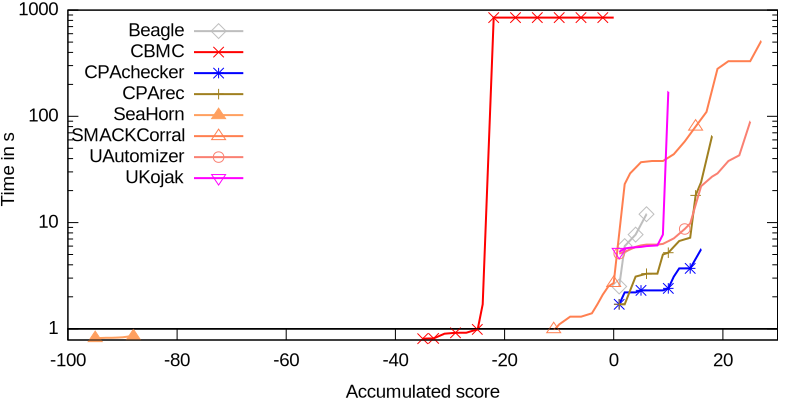
\includegraphics[width=\textwidth]{fig/competition-result}
  \caption{Accumulated Score over Time}
  \label{figure:accumulated-score}
\end{figure}


%%% Local Variables: 
%%% mode: latex
%%% TeX-master: "draft"
%%% LaTeX-command: "latex -shell-escape"
%%% End: 

\end{comment}